\begin{enunciado}{\ejercicio}
  \begin{enumerate}[label=\alph*)]
    \item Calcular $w + \conj w + (w + w^2)^2 - w^{38}(1 - w^2)$ para cada $w \en G_7$.
    \item Calcular $w^{73} + \conj w \cdot w^9 + 8$ para cada $w\en G_3$.
    \item Calcular $1 + w^2 + w^{-2} + w^4 + w^{-4}$ para cada $w\en G_{10}$.
    \item Calcular $w^{14} + w^{-8} + \conj w^4 + \conj{w^{-3}}$ para cada $w \en G_5$
  \end{enumerate}
\end{enunciado}

\textit{Voy a estar usando las siguientes propiedades en $G_n$: }\\
Si $w \en G_n \entonces
  \llave{l}{
    w^n = 1 \entonces w^k = w^{r_n(k)}                                                                         \\
    \conj w^k = w^{r_n(-k)}                                                                                    \\
    \sumatoria{k=0}{n-1}w^k = 0                                                                                \\
    m \divideA n \entonces G_m \subseteq G_n,\text{ lo uso para saber con cuales raíces hay que tener cuidado} \\
    \text{Si } w \en G_p \text{ con $p$ primo }}$\par

\begin{enumerate}[label=\alph*)]
  \item Calcular $w + \conj w + (w + w^2)^2 - w^{38}(1 - w^2)$ para cada $w \en G_7$.

        \separadorCorto
        Raíces de $G_7$ de interés: 7 es primo e impar $\entonces w = 1$ se hace a parte.\par
        \textit{Si} $w = 1$: \par
        $w + \conj w + (w + w^2)^2 - w^{38}(1 - w^2) = 6$\par

        \textit{Si} $w \distinto 1$: \\
        $w + \ub{\conj w}{w^6} + (w + w^2)^2 - w^{38}(1 - w^2) =
          w + w^6 + w^2 + 2w^3 + w^4 - \ub{(w^7)^5}{=1} w^3(1 - w^2) =\\
          =  \magenta{-1} + \ub{\magenta{1} + w + w^2 + w^3 + w^4 + w^5 + w^6}{=0} = -1 \Tilde$

  \item Calcular $w^{73} + \conj w \cdot w^9 + 8$ para cada $w\en G_3$.

        \separadorCorto
        Raíces de $G_3$ de interés: 3 es primo e impar $\entonces w = 1$ se hace a parte.\par
        \textit{Si} $w = 1$: \par
        $w^{73} + \conj w \cdot w^9 + 8 = 10 $\par

        \textit{Si} $w \distinto 1$: \\
        $\ub{w^{73}}{w} + \ub{\conj w \cdot w^9 }{w^2 \cdot 1}+ 8 =
          \magenta{-1} + \ub{\magenta{1} + w + w^2}{= 0} + 8 = 7 $

  \item Calcular $1 + w^2 + w^{-2} + w^4 + w^{-4}$ para cada $w\en G_{10}$.
        \separadorCorto
        Raíces de $G_{10}$ de interés: $2 \divideA 10 \ytext 5 \divideA 10$. $10$ es par $\entonces w = \pm1$ y
        raíces de $G_2$ y de $G_5$ se hacen a parte.\par

        \begin{minipage}{0.55\textwidth}
          \begin{itemize}
            \item \textit{Si} $w = \pm1$: \par
                  $1 + w^2 + w^{-2} + w^4 + w^{-4} = 5$ \Tilde\par

            \item \textit{Si} $w \en G_{10} \ytext w \distinto \pm 1$: \par
                  $ 1 + w^2 + w^{-2} + w^4 + w^{-4} = 1 + w^2 + w^8 + w^4 + w^6 =\\
                    = \sumatoria{k=0}{4} (w^2)^k = \frac{(w^2)^5 - 1}{w^2 - 1} =
                    \frac{\ob{\scriptstyle w^{10}}{=1} - 1}{w^2 - 1} = 0$
          \end{itemize}
        \end{minipage}
        \begin{minipage}{0.3\textwidth}
          \centering
          $G_5 \subseteq G_{10}$\par
          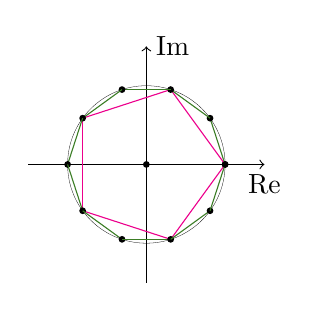
\begin{tikzpicture}[baseline=0]
            \draw[->] (-1.5,0) -- (1.5,0) node[below] {Re};
            \draw[->] (0,-1.5) -- (0,1.5) node[right] {Im};
            \draw[ultra thin] (0,0) circle (1);
            \filldraw[thin] (0,0) circle (1pt); % Added the origin
            \foreach \x in {0,...,10} {
                \filldraw (\x*360/10:1) circle (1pt);
                \ifnum\x<10
                  \draw[OliveGreen] (\x*360/10:1) -- ({(\x+1)*360/10}:1);
                \fi
                \ifnum\x<5
                  \draw[magenta] (\x*360/5:1) -- ({(\x+1)*360/5}:1);
                \fi
              }
          \end{tikzpicture}

          $"G_5" \subseteq G_{10}$\par
          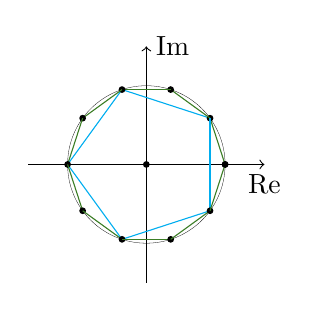
\begin{tikzpicture}[baseline=0]
            \draw[->] (-1.5,0) -- (1.5,0) node[below] {Re};
            \draw[->] (0,-1.5) -- (0,1.5) node[right] {Im};
            \draw[ultra thin] (0,0) circle (1);
            \filldraw[thin] (0,0) circle (1pt); % Added the origin

            \foreach \x in {0,...,10} {
                \filldraw (\x*360/10:1) circle (1pt);
                \ifnum\x<10
                  \draw[OliveGreen] (\x*360/10:1) -- ({(\x+1)*360/10}:1);
                \fi
                \ifnum\x<5
                  \draw[cyan] ({\x*360/5+360/10}:1) -- ({(\x+1)*360/5+360/10}:1);
                \fi
              }
          \end{tikzpicture}
        \end{minipage}

  \item Calcular $w^{14} + w^{-8} + \conj w^4 + \conj{w^{-3}}$ para cada $w \en G_5$

        \separadorCorto
        \textit{Si} $w = 1$: \par
        $w^{14} + w^{-8} + \conj w^4 + \conj{w^{-3}} = 4$

        \textit{Si} $w \distinto 1$: \par
        $w^{14} + w^{-8} + \conj w^4 + \conj{w^{-3}} =
          w^4 + w^2 + w + w^3 =
          \magenta{-1} + \ub{\magenta{1} + w + w^2 + w^3 + w^4}{= 0} = -1 $

\end{enumerate}
